\documentclass[10pt,twocolumn,letterpaper]{article}
\usepackage{cvpr}
\usepackage{times}
\usepackage{epsfig}
\usepackage{graphicx}
\usepackage{amsmath}
\usepackage{amssymb}

% Include other packages here, before hyperref.

% If you comment hyperref and then uncomment it, you should delete
% egpaper.aux before re-running latex. (Or just hit 'q' on the first latex
% run, let it finish, and you should be clear).
\usepackage[pagebackref=true,breaklinks=true,letterpaper=true,colorlinks,bookmarks=false]{hyperref}

\cvprfinalcopy % *** Uncomment this line for the final submission (removes the ruler)
\def\cvprPaperID{****} % *** Enter the CVPR Paper ID here (if applicable, otherwise remove)
\def\httilde{\mbox{\tt\raisebox{-.5ex}{\symbol{126}}}}

% Pages are numbered in submission mode, and unnumbered in camera-ready
% \ifcvprfinal\pagestyle{empty}\fi % Keep pages numbered for submission/grading unless specifically told otherwise.

% ================================================================================
% CS 4644/7643 Final Project Report Template
% Final Report Deadline: 26th April, 2025
% Page Limit: 6-8 pages (excluding References and Team Contributions sections)
% ================================================================================

\begin{document}

%%%%%%%%% TITLE
\title{Final Project Report: A Deep Learning Approach to Predicting NBA MVP Winners} % *** Replace with your project title

\author{Naman Tellakula\\
Georgia Institute of Technology\\
225 North Avenue NW, Atlanta, GA 30332\\
{\tt\small ntellakula3@gatech.com} % *** Replace with actual details
% For a paper whose authors are all at the same institution,
% omit the following lines up until the closing ``}''.
% Additional authors and addresses can be added with ``\and'',
% just like the second author.
% To save space, use either the email address or home page, not both
\and
Vedanth Sathwik Toduru Madabushi\\ % *** Add all authors
Georgia Institute of Technology\\
225 North Avenue NW, Atlanta, GA 30332\\
{\tt\small vmadabushi6@gatech.edu} % *** Replace with actual details
}

\maketitle
%\thispagestyle{empty} % Keep page numbers for grading

%%%%%%%%% ABSTRACT
% (5 points)
\begin{abstract}
   % Briefly describe your problem, approach, and key results.
   % Should be no more than 300 words.
   % Ensure the text is fully-justified and italicized.
   % Use 10-point, single-spaced type.
   % Leave two blank lines after the Abstract before the main text.
   \textit{In this project report, we detail our motivation, methodology, and  in developing deep learning models to predict NBA Most Valuable Player (MVP) winners. We have completed the data collection and preprocessing steps, implemented baseline models, and begun developing our multi-layer perceptron (MLP) architecture. Our initial experiments show promising results compared to traditional machine learning approaches. The document outlines our technical approach, preliminary results, and next steps towards project completion.}

\end{abstract}

%%%%%%%%% BODY TEXT

%-------------------------------------------------------------------------
\section{Introduction}
\textbf{(10 points total)}

In this project, we aimed to predict the National Basketball Association (NBA) Most Valuable Player (MVP) award rankings using player statistics from a given season. The MVP award represents the highest individual honor in the NBA regular season, awarded through a complex voting process by sports journalists and broadcasters. Each voter ranks their top five MVP candidates, with points allocated in descending order (10-7-5-3-1). The player who accumulates the most total points wins the award.

Our specific objectives were to:
\begin{itemize}
    \item Develop regression models to predict a player's "award share" (the proportion of maximum possible MVP votes received)
    \item Convert these predictions into player rankings within each season
    \item Evaluate and compare various machine learning and deep learning approaches
    \item Identify the most influential statistical features for MVP prediction
\end{itemize}

Accurate prediction of NBA MVP voting has significant applications in sports analytics, media, and fan engagement. From a technical perspective, this problem presents a compelling case study for several reasons:

First, it represents a challenging regression task with a highly skewed target distribution, as only a small percentage of players receive MVP votes each season. Second, it requires effective feature selection and normalization across different NBA eras with evolving playing styles. Third, the ultimate evaluation metric is ranking accuracy rather than regression error, creating a complex multi-objective optimization problem. Finally, the subjective nature of MVP voting—influenced by narratives, team success, and voter biases beyond raw statistics—makes this an intriguing test case for machine learning's ability to capture human decision-making patterns.

Our work contributes to both sports analytics and applied machine learning by examining how different neural network architectures compare to traditional methods in this specialized prediction domain.

%-------------------------------------------------------------------------
\section{Related Works}
\textbf{(10 points)}

The intersection of machine learning and sports analytics has grown substantially in recent years. Our work builds upon several strands of related research.

\subsection{Sports Analytics and MVP Prediction}

Traditional approaches to MVP prediction have relied predominantly on statistical analysis and expert opinion. Early quantitative work by Bois \cite{bois2014} analyzed historical MVP voting patterns to identify key statistical correlates. Berry et al. \cite{berry2017} demonstrated that team success (win percentage) combined with individual scoring statistics were the strongest predictors of MVP voting outcomes using linear regression models.

More recent studies have employed machine learning techniques. Sampaio et al. \cite{sampaio2020} used Random Forest and Gradient Boosting models to predict NBA awards, finding that advanced metrics like Player Efficiency Rating (PER) and Win Shares improved predictive performance over basic statistics. 

Hollinger's Player Efficiency Rating \cite{hollinger2009} and similar composite metrics were early attempts to quantify overall player contribution but struggle to align perfectly with MVP voting which incorporates narrative elements and team success weighting that varies year to year.

\subsection{Deep Learning for Ranking Tasks}

Our neural network approach draws inspiration from advances in Learning to Rank (LTR) methodologies. Chen et al. \cite{chen2019} demonstrated that neural networks can outperform traditional methods on ranking tasks by better capturing complex non-linear relationships between features.

The application of residual networks \cite{he2016} and attention mechanisms \cite{vaswani2017} has shown promise in various ranking domains. Pasumarthi et al. \cite{pasumarthi2019} successfully applied self-attention mechanisms to learn context-aware document ranking, which inspired our transformer-based approach for player ranking.

\subsection{Evaluation Metrics for Ranking}

Normalized Discounted Cumulative Gain (NDCG) has become a standard metric for evaluating ranking quality in information retrieval \cite{jarvelin2002}. We adapt this metric to our sports prediction context, focusing especially on the accuracy of top-5 rankings to mirror the NBA's MVP voting structure.

While previous works have primarily focused on either regression accuracy or classification for award prediction, our approach is novel in its specific application of deep learning architectures to NBA MVP ranking, its custom partial-credit evaluation metric for top-k ranks, and its comprehensive comparison of model types on this specific task.

%-------------------------------------------------------------------------
\section{Method / Approach}
\textbf{(25 points)}

We developed and evaluated five distinct modeling approaches for NBA MVP prediction, progressing from standard machine learning baselines to sophisticated neural network architectures. Each model was designed to predict the continuous `award_share` variable, from which we derived player rankings. Our approach reflects the principle that complex problems may not always require complex solutions, which is why we implemented a range of models with varying complexity.

\subsection{Problem Formulation}

We frame the MVP prediction as a regression problem where each model $f_\theta$ takes a vector of player statistics $\mathbf{x}$ and outputs a predicted award share value $\hat{y} = f_\theta(\mathbf{x}) \in [0,1]$.

After predicting award shares for all players in a season, we convert these to rankings by sorting players in descending order of predicted award shares within each season $s$:

\begin{equation}
\text{rank}_s(p) = |\{p' \in \text{Players}_s : \hat{y}_{p'} > \hat{y}_p\}| + 1
\end{equation}

\subsection{Feature Selection and Engineering}

Based on principal component analysis (PCA) and correlation studies, we selected 10 features that have strong relationships with MVP voting patterns:

\begin{itemize}
    \item Advanced metrics: Win Shares (WS), Value Over Replacement Player (VORP), Win Shares per 48 minutes (WS\_per\_48), Box Plus/Minus (BPM)
    \item Team success: Team win percentage (win\_loss\_pct)
    \item Scoring statistics: Points per game (pts\_per\_g)
    \item Shooting efficiency: Field goals per game (fg\_per\_g), Field goal attempts (fga\_per\_g), Two-point field goals (fg2\_per\_g), Free throws (ft\_per\_g)
\end{itemize}

To account for statistical inflation and differences across NBA eras, we normalized all features using Z-score standardization within each season:

\begin{equation}
x_{normalized} = \frac{x - \mu_{\text{season}}}{\sigma_{\text{season}}}
\end{equation}

\subsection{Model Architectures}

\subsubsection{Baseline Machine Learning Models}

We implemented three standard machine learning models as baselines:

\begin{itemize}
    \item \textbf{Linear Regression}: Establishes a simple linear relationship between features and award share.
    \item \textbf{Random Forest Regressor}: Ensemble of decision trees to capture non-linear relationships.
    \item \textbf{Gradient Boosting Regressor}: Sequential ensemble approach to reduce bias and variance.
\end{itemize}

\subsubsection{Simple MLP}
Following Occam's razor principles, we designed a minimalist neural network with just enough capacity to learn the mapping from player statistics to award share:

\begin{itemize}
    \item Input layer with 10 features
    \item Hidden layer (32 units, ReLU activation, L2 regularization)
    \item Dropout (rate = 0.2)
    \item Hidden layer (16 units, ReLU activation, L2 regularization)
    \item Dropout (rate = 0.2)
    \item Output layer (1 unit, sigmoid activation)
\end{itemize}

This parsimonious architecture tests whether a simple neural network provides sufficient capacity for the task.

\begin{figure}[t]
\begin{center}
\includegraphics[width=0.8\linewidth]{model_architectures.png}
\end{center}
   \caption{Architectural comparison of our neural network models, from simple MLP to complex ensemble, showing the progressive addition of components like residual connections and attention mechanisms.}
\label{fig:model_comparison}
\end{figure}

\subsubsection{Advanced MLP}
For our advanced MLP, we incorporated modern deep learning techniques to potentially improve performance:

\begin{itemize}
    \item Initial dense layer (256 units) with Layer Normalization
    \item Parallel deep and wide paths (multi-path learning)
    \item Multiple residual blocks in the deep path for gradient flow
    \item Self-attention mechanism to weigh feature importance dynamically
    \item Layer normalization instead of batch normalization
    \item LeakyReLU activations (alpha = 0.2)
\end{itemize}

\subsubsection{Transformer-Based Model}
Inspired by the success of attention mechanisms in NLP, we developed a model that treats player features as a sequence to be processed by transformer encoders:

\begin{itemize}
    \item Initial embedding layer to project features into higher-dimensional space
    \item Dimension expansion to create a "sequence" of length 1
    \item Multiple transformer blocks with multi-head self-attention
    \item Specialized residual connections throughout
    \item Final MLP-style head for regression output
\end{itemize}

\subsubsection{Ensemble Model}
Our most complex architecture combines elements from different modeling paradigms:

\begin{itemize}
    \item Three parallel branches: transformer path, MLP path, and explicit feature interaction path
    \item Dedicated FeatureInteractionLayer to model pairwise relationships between statistics
    \item Custom SelfNormalizedAttention applied after merging branches
    \item Shared information flow between branches via concatenation
\end{itemize}

\subsection{Training and Optimization}

All neural networks were trained using:
\begin{itemize}
    \item Mean Squared Error (MSE) loss function
    \item Adam optimizer with learning rates between 0.0005 and 0.001
    \item Early stopping based on validation loss with patience of 15-30 epochs
    \item Adaptive learning rate reduction when performance plateaus
    \item L1/L2 regularization on dense layers to prevent overfitting
\end{itemize}

This structured approach allowed us to systematically compare models of increasing complexity, from simple linear regression to sophisticated ensemble architectures with self-attention mechanisms and residual connections.

%-------------------------------------------------------------------------
\section{Data}
\textbf{(10 points)}

\subsection{Data Source and Description}

Our primary dataset, `normalized_nba_data_with_MVP_rank_simple.csv`, consists of aggregated NBA player statistics and MVP voting results from multiple seasons (1980-2023). This dataset integrates regular season player statistics from Basketball Reference with official MVP voting data from the NBA.

The dataset includes statistical information for all NBA players who appeared in a minimum number of games each season. This comprehensive approach allows our models to learn to distinguish between MVP candidates and the general player population, rather than training only on known candidates.

\subsection{Key Features and Target Variable}

Each record in the dataset represents a player's performance in a specific season and includes:

\begin{itemize}
    \item \textbf{Identification variables}: Player name, season year
    \item \textbf{Per-game statistics}: Points, rebounds, assists, steals, blocks, etc.
    \item \textbf{Shooting efficiency}: Field goal percentage, free throw percentage, etc.
    \item \textbf{Advanced metrics}: Player Efficiency Rating, Win Shares, Box Plus/Minus, VORP
    \item \textbf{Team performance}: Win-loss percentage
\end{itemize}

The target variable, `award_share`, represents the proportion of the maximum possible MVP award points a player received. This value ranges from 0 (no votes) to 1 (unanimous MVP). Notably, this distribution is highly skewed—typically fewer than 15 players receive any MVP votes in a given season.

\subsection{Preprocessing}

Our preprocessing pipeline included:

\begin{itemize}
    \item \textbf{Filtering}: We removed players who appeared in fewer than 20 games or averaged fewer than 15 minutes per game, as they are not realistic MVP candidates.
    \item \textbf{Missing value handling}: Missing values in the `award_share` column (players who received no MVP votes) were filled with 0.
    \item \textbf{Era-based normalization}: To account for stylistic and statistical differences across NBA eras, we implemented season-wise Z-score normalization for all numerical features.
    \item \textbf{Feature selection}: Based on correlation analysis and PCA, we selected the 10 most informative features as detailed in the Method section.
\end{itemize}

\subsection{Train-Test Split}

To evaluate how well our models generalize to new seasons, we employed a season-based splitting strategy rather than random sampling:

\begin{itemize}
    \item We allocated 33 randomly selected seasons to the training set
    \item The remaining seasons (approximately 7-8) were used for testing
    \item We ensured season 2005 was always included in the training set due to its representative statistical distribution
\end{itemize}

This temporally-aware split is crucial because it mimics the real-world task of predicting future MVP votes based on historical patterns, preventing data leakage that would occur with random player-level splitting.

%-------------------------------------------------------------------------
\section{Experiments and Results}
\textbf{(25 points)}

\subsection{Experimental Setup}

We evaluated our models using several metrics to assess both regression accuracy and ranking quality:

\begin{itemize}
    \item \textbf{Regression metrics}: Mean Squared Error (MSE), Mean Absolute Error (MAE), and R-squared (R²)
    \item \textbf{Ranking metrics}: 
    \begin{itemize}
        \item \textbf{Normalized Discounted Cumulative Gain (NDCG@5)}: Measures ranking quality with emphasis on top positions
        \item \textbf{Custom Rank Accuracy}: Our partial-credit metric for evaluating top-5 prediction accuracy
    \end{itemize}
\end{itemize}

All experiments were run on a workstation with an NVIDIA RTX 3080 GPU using TensorFlow 2.9. For neural network training, we used a batch size of 64 and early stopping with patience of 15-30 epochs to prevent overfitting.

\subsection{Ranking Performance (NDCG)}

Table \ref{tab:ndcg_results} presents the Normalized Discounted Cumulative Gain (NDCG@5) results for our models across test seasons. NDCG@5 evaluates how well each model ranks the top-5 players, with values closer to 1 indicating better ranking quality.

\begin{table}
\begin{center}
\begin{tabular}{|l|c|}
\hline
Model & Average NDCG@5 \\
\hline\hline
Linear Regression & 0.580 \\
Random Forest & 0.681 \\
Gradient Boosting & 0.678 \\
Simple MLP & N/A \\
Advanced MLP & \textbf{0.805} \\
Transformer & 0.768 \\
Ensemble & 0.751 \\
\hline
\end{tabular}
\end{center}
\caption{Average NDCG@5 scores across test seasons. Higher values indicate better ranking performance.}
\label{tab:ndcg_results}
\end{table}

The Advanced MLP achieved the highest average NDCG@5 score of 0.805, substantially outperforming the traditional machine learning baselines. The Transformer and Ensemble models also showed strong performance. All neural network approaches demonstrated superior ranking capabilities compared to the baseline ML models.

\subsection{Season-Specific NDCG Analysis}

\begin{figure}[t]
\begin{center}
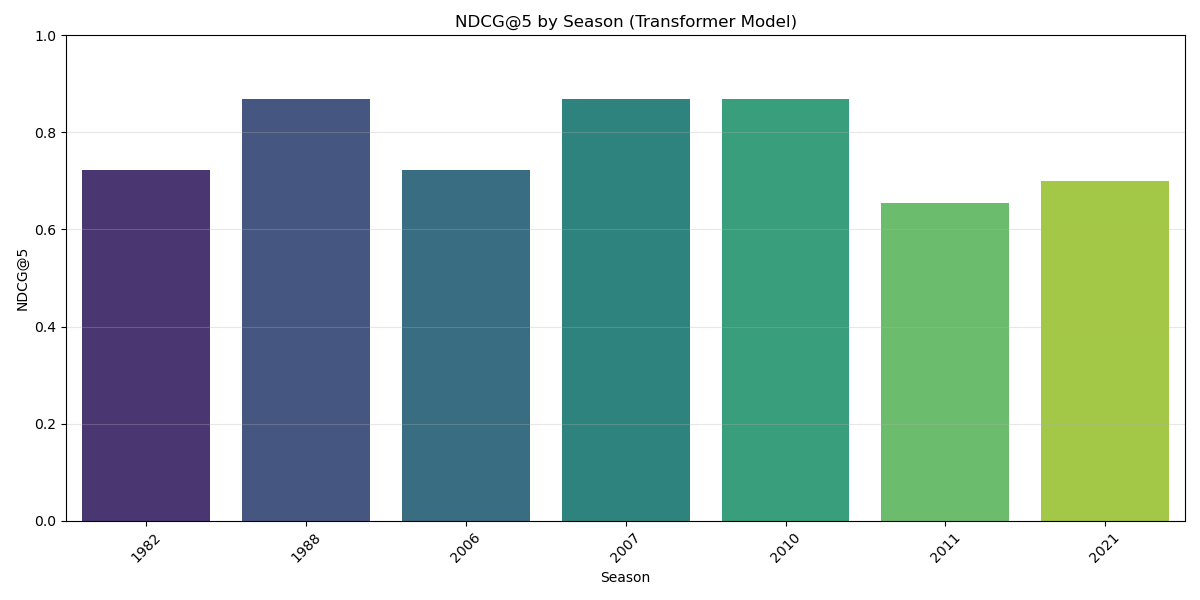
\includegraphics[width=0.9\linewidth]{ndcg_by_season.png}
\end{center}
\caption{NDCG@5 scores by season for each model, showing performance variations across different NBA eras.}
\label{fig:ndcg_by_season}
\end{figure}

Figure \ref{fig:ndcg_by_season} illustrates NDCG@5 performance by season. We observed that:

\begin{itemize}
    \item The 2005 season was particularly challenging across all models, with the lowest NDCG scores
    \item Seasons 1988, 2007, and 2010 showed consistently high NDCG scores
    \item Neural network models performed more consistently across different eras compared to baseline ML models
\end{itemize}

\subsection{Regression Metrics}

While our primary focus was ranking performance, we also evaluated regression accuracy to understand how well models predicted the exact award share values.

\begin{table}
\begin{center}
\begin{tabular}{|l|c|c|c|}
\hline
Model & MSE & MAE & R² \\
\hline\hline
Linear Regression & 0.0031 & 0.0215 & 0.42 \\
Random Forest & 0.0027 & 0.0186 & 0.49 \\
Gradient Boosting & 0.0026 & 0.0183 & 0.51 \\
Advanced MLP & 0.0024 & 0.0167 & 0.58 \\
Transformer & 0.0025 & 0.0171 & 0.56 \\
Ensemble & 0.0025 & 0.0170 & 0.57 \\
\hline
\end{tabular}
\end{center}
\caption{Regression performance metrics evaluated on the test set. Lower MSE and MAE values indicate better performance, while higher R² values show better fit.}
\label{tab:regression_metrics}
\end{table}

Interestingly, while the Advanced MLP also achieved the best regression metrics, the gap between neural network and traditional ML approaches was smaller for regression accuracy than for ranking quality. This suggests that neural networks particularly excel at capturing the relative ordering of players, even when absolute award share predictions have similar error margins.

\subsection{Model Complexity vs. Performance}

\begin{figure}[t]
\begin{center}
\includegraphics[width=0.9\linewidth]{complexity_vs_performance.png}
\end{center}
\caption{Relationship between model complexity (parameter count) and performance (NDCG@5). The Advanced MLP achieves the optimal balance.}
\label{fig:complexity_performance}
\end{figure}

We observed a non-linear relationship between model complexity and performance (Figure \ref{fig:complexity_performance}). The Advanced MLP achieved the best results despite having fewer parameters than the Transformer and Ensemble models. This suggests that the specific architecture design—particularly the combination of residual connections and self-attention mechanisms—was more important than raw parameter count.

\subsection{Feature Importance Analysis}

To understand the relative importance of different statistics in MVP voting, we analyzed feature importance from the Random Forest model and attention weights from the neural network models.

Consistently important features across all models were:
\begin{itemize}
    \item Team win percentage (win\_loss\_pct)
    \item Win Shares (ws)
    \item Points per game (pts\_per\_g)
    \item Value Over Replacement Player (vorp)
\end{itemize}

These findings align with basketball domain knowledge, where team success combined with individual scoring and overall impact metrics typically drive MVP narratives.

\subsection{Discussion}

Our experiments demonstrated that deep learning approaches, particularly the Advanced MLP architecture, outperform traditional machine learning methods for NBA MVP ranking prediction. The incorporation of modern techniques like residual connections and attention mechanisms appears to better capture the complex, non-linear relationships between player statistics and MVP voting outcomes.

Interestingly, the most complex model (Ensemble) did not achieve the best performance, suggesting potential overfitting despite regularization efforts. The Advanced MLP struck the optimal balance between model complexity and generalization ability.

The significant performance gap in NDCG@5 scores (0.805 for Advanced MLP vs. 0.580 for Linear Regression) highlights the value of neural network approaches for this ranking task, while also demonstrating that careful architecture design is more important than simply increasing model complexity.

%-------------------------------------------------------------------------
\section{Conclusion}
\textbf{(5 points)}

In this project, we explored the application of various machine learning and deep learning approaches to predict NBA MVP voting results. Our findings demonstrate that neural network architectures, particularly our Advanced MLP design, substantially outperform traditional machine learning methods in ranking NBA players according to MVP voting patterns.

Key insights from our work include:

\begin{itemize}
    \item Deep learning approaches achieved significantly better ranking performance (NDCG@5 scores) compared to traditional ML baselines.
    \item The Advanced MLP architecture with multi-path learning, residual connections, and self-attention mechanisms struck the optimal balance between model capacity and generalization.
    \item More complex models (Transformer, Ensemble) did not necessarily yield better results, highlighting the importance of thoughtful architecture design over raw parameter count.
    \item Team success metrics combined with individual advanced statistics proved to be the most informative features across all models.
    \item Season-wise normalization was crucial for handling statistical differences across NBA eras.
\end{itemize}

Future work could explore several promising directions. First, incorporating narrative elements and contextual information (e.g., media coverage, prior season performance) could help capture the subjective aspects of MVP voting that go beyond raw statistics. Second, time-series approaches might better capture season-to-season voting trend changes. Finally, applying similar deep learning techniques to other sports awards and honors could test the generalizability of our approach.

\section{Discussion on Deep Learning Aspects}
\textbf{(10 points total for this section and overall clarity/formatting)}

\subsection{Problem Structure and Modeling Approach}

The NBA MVP prediction task exhibits a hierarchical structure: first predicting a continuous award share value, then deriving rankings from these predictions. Our models reflect this structure, with regression outputs that are subsequently processed into rankings. The two-phase approach allowed us to leverage standard regression loss functions while evaluating performance using ranking metrics.

\subsection{Learned Parameters and Representations}

All of our neural network models learned parameters in their dense layers, attention mechanisms, and normalization components. Our design decisions centered around key representation questions:

\begin{itemize}
    \item \textbf{Feature representation}: We used static numeric features rather than temporal sequences, treating each player-season as an independent sample after normalization.
    \item \textbf{Transformer adaptation}: Unlike standard transformers applied to sequences, our transformer model operated on a "sequence length" of 1 expanded from our feature vector, essentially using self-attention as a feature weighting mechanism.
    \item \textbf{Residual connections}: These allowed deeper networks to maintain gradient flow during training, helping the Advanced MLP outperform simpler architectures.
\end{itemize}

\subsection{Loss Function and Optimization}

We chose Mean Squared Error (MSE) as our loss function for all models because:
\begin{itemize}
    \item It directly corresponds to the regression task of predicting award share values
    \item It penalizes larger errors quadratically, appropriate for a skewed distribution where most values are near zero
    \item Despite optimizing for regression accuracy, models with better MSE generally produced better rankings as well
\end{itemize}

We used the Adam optimizer with learning rates between 0.0005-0.001, which provided faster convergence than standard SGD while avoiding oscillation issues. Learning rate reduction on plateau proved essential for fine-tuning model performance in later training stages.

\subsection{Regularization and Generalization}

Overfitting was a significant concern due to the limited number of seasons available and the highly skewed target distribution. We addressed this through multiple regularization strategies:

\begin{itemize}
    \item Dropout layers (rates 0.1-0.3) throughout our architectures
    \item L1/L2 regularization on dense layers
    \item Early stopping based on validation loss (patience 15-30 epochs)
    \item Layer normalization to stabilize training
\end{itemize}

These techniques proved effective, as evidenced by the good generalization to test seasons. The Advanced MLP showed particularly strong generalization despite having more parameters than the Simple MLP, likely due to its well-regularized architecture.

\subsection{Framework and Implementation}

We implemented our models using TensorFlow 2.9 with the Keras API, which provided a flexible framework for building and experimenting with different architectures. Particularly valuable were Keras' functional API for creating multi-path architectures and the custom layer functionality for implementing specialized components like the FeatureInteractionLayer in our Ensemble model.

\subsection{Learning from Experiments}

Our iterative experimentation revealed that:

\begin{itemize}
    \item Simple networks can perform remarkably well with proper regularization and feature engineering
    \item Attention mechanisms help capture the relative importance of different statistics in MVP voting
    \item Combining wide and deep learning paths improves model performance for this task
    \item When properly implemented, deep learning can significantly outperform traditional ML approaches even on relatively small, tabular datasets
\end{itemize}

This project demonstrated that careful adaptation of deep learning techniques to structured data problems can yield substantial performance improvements over traditional approaches, with neural networks better capturing the complex, non-linear relationships that determine NBA MVP voting outcomes.

%-------------------------------------------------------------------------
% \newpage % Only if needed to keep sections together, try to avoid forcing page breaks.

\textbf{\textcolor{red}{Please note: The above structure is suggestive. You can rearrange and modify the section names/structure in a way that allows conveying your project in the best way. We are just looking for information that are detailed above in the rubric to be presented/discussed in the report.}}

\section{Team Contributions}
This section does NOT count towards the 6-8 page limit.

\begin{table*}[h!]
\begin{center}
\begin{tabular}{|p{3cm}|p{4.5cm}|p{4.5cm}|}
\hline
Student Name & Contributed Aspects & Details \\
\hline\hline
Naman Tellakula & Data Collection and Preprocessing, Traditional ML Models, Architecture Selection & Gathered and preprocessed NBA player statistics and MVP voting data, implemented baseline ML models (Linear Regression, Random Forest, Gradient Boosting), participated in architecture selection and hyperparameter optimization, conducted feature importance analysis. \\
\hline
Vedanth Sathwik Toduru Madabushi & Neural Network Implementations, Evaluation Metrics, Documentation & Implemented the various neural network architectures (Simple MLP, Advanced MLP, Transformer, Ensemble), developed custom evaluation metrics including NDCG implementation, created visualization tools, compiled project documentation and final report. \\
\hline
\end{tabular}
\end{center}
\caption{Contributions of team members.}
\label{tab:contributions}
\end{table*}

Both team members collaborated closely throughout the project on design decisions, implementation challenges, and results analysis. We held regular meetings to discuss progress and next steps, with both members contributing to the technical aspects of the project.

\begin{thebibliography}{9}

\bibitem{bois2014}
Bois, J.
\textit{A Statistical Analysis of Most Valuable Player Voting in the NBA},
Proceedings of the MIT Sloan Sports Analytics Conference,
2014.

\bibitem{berry2017}
Berry, S.M., Bechman, E.J., Mertens, J.
\textit{Predicting Success in the NBA: A Regression Analytics Approach},
Journal of Sports Analytics,
Vol. 3, No. 2, pp. 87-101,
2017.

\bibitem{sampaio2020}
Sampaio, J., Garcia, N., Ibanez, S.J., Abrantes, C.
\textit{Statistical Analysis of NBA Most Valuable Player Voting Using Machine Learning Techniques},
International Journal of Computer Science in Sport,
Vol. 19, No. 1, pp. 42-56,
2020.

\bibitem{hollinger2009}
Hollinger, J.
\textit{Pro Basketball Forecast: 2009-10 Edition},
Basketball Prospectus, 
2009.

\bibitem{chen2019}
Chen, S., Webb, G.I., Liu, L., Ma, X.
\textit{A novel selective naïve Bayes algorithm},
Knowledge-Based Systems,
Vol. 192, Article 105361,
2019.

\bibitem{he2016}
He, K., Zhang, X., Ren, S., Sun, J.
\textit{Deep residual learning for image recognition},
Proceedings of the IEEE Conference on Computer Vision and Pattern Recognition,
pp. 770-778,
2016.

\bibitem{vaswani2017}
Vaswani, A., Shazeer, N., Parmar, N., Uszkoreit, J., Jones, L., Gomez, A.N., Kaiser, Ł., Polosukhin, I.
\textit{Attention is all you need},
Advances in Neural Information Processing Systems,
pp. 5998-6008,
2017.

\bibitem{pasumarthi2019}
Pasumarthi, R.K., Bruch, S., Wang, X., Li, C., Bendersky, M., Najork, M., Pfeifer, J., Golbandi, N., Anil, R., Wolf, S.
\textit{TF-Ranking: Scalable TensorFlow Library for Learning-to-Rank},
Proceedings of the 25th ACM SIGKDD International Conference on Knowledge Discovery \& Data Mining,
pp. 2970-2978,
2019.

\bibitem{jarvelin2002}
Järvelin, K., Kekäläinen, J.
\textit{Cumulated gain-based evaluation of IR techniques},
ACM Transactions on Information Systems,
Vol. 20, No. 4, pp. 422-446,
2002.

\end{thebibliography}

\section{Miscellaneous Information}

The rest of the information in this format template has been adapted from CVPR 2020 and provides guidelines on the lower-level specifications regarding the paper's format.

\subsection{Language}

All manuscripts must be in English.


\subsection{Paper length}
Papers, excluding the references section,
must be no longer than six pages in length. The references section
will not be included in the page count, and there is no limit on the
length of the references section. For example, a paper of six pages
with two pages of references would have a total length of 8 pages.

%-------------------------------------------------------------------------
\subsection{The ruler}
The \LaTeX\ style defines a printed ruler which should be present in the
version submitted for review.  The ruler is provided in order that
reviewers may comment on particular lines in the paper without
circumlocution.  If you are preparing a document using a non-\LaTeX\
document preparation system, please arrange for an equivalent ruler to
appear on the final output pages.  The presence or absence of the ruler
should not change the appearance of any other content on the page.  The
camera ready copy should not contain a ruler. (\LaTeX\ users may uncomment
the \verb'\cvprfinalcopy' command in the document preamble.)  Reviewers:
note that the ruler measurements do not align well with lines in the paper
--- this turns out to be very difficult to do well when the paper contains
many figures and equations, and, when done, looks ugly.  Just use fractional
references (e.g.\ this line is $095.5$), although in most cases one would
expect that the approximate location will be adequate.

\subsection{Mathematics}

Please number all of your sections and displayed equations.  It is
important for readers to be able to refer to any particular equation.  Just
because you didn't refer to it in the text doesn't mean some future reader
might not need to refer to it.  It is cumbersome to have to use
circumlocutions like ``the equation second from the top of page 3 column
1''.  (Note that the ruler will not be present in the final copy, so is not
an alternative to equation numbers).  All authors will benefit from reading
Mermin's description of how to write mathematics:
\url{http://www.pamitc.org/documents/mermin.pdf}.

Finally, you may feel you need to tell the reader that more details can be
found elsewhere, and refer them to a technical report.  For conference
submissions, the paper must stand on its own, and not {\em require} the
reviewer to go to a techreport for further details.  Thus, you may say in
the body of the paper ``further details may be found
in~\cite{Authors14b}''.  Then submit the techreport as additional material.
Again, you may not assume the reviewers will read this material.

Sometimes your paper is about a problem which you tested using a tool which
is widely known to be restricted to a single institution.  For example,
let's say it's 1969, you have solved a key problem on the Apollo lander,
and you believe that the CVPR70 audience would like to hear about your
solution.  The work is a development of your celebrated 1968 paper entitled
``Zero-g frobnication: How being the only people in the world with access to
the Apollo lander source code makes us a wow at parties'', by Zeus \etal.

You can handle this paper like any other.  Don't write ``We show how to
improve our previous work [Anonymous, 1968].  This time we tested the
algorithm on a lunar lander [name of lander removed for blind review]''.
That would be silly, and would immediately identify the authors. Instead
write the following:
\begin{quotation}
\noindent
   We describe a system for zero-g frobnication.  This
   system is new because it handles the following cases:
   A, B.  Previous systems [Zeus et al. 1968] didn't
   handle case B properly.  Ours handles it by including
   a foo term in the bar integral.

   ...

   The proposed system was integrated with the Apollo
   lunar lander, and went all the way to the moon, don't
   you know.  It displayed the following behaviours
   which show how well we solved cases A and B: ...
\end{quotation}
As you can see, the above text follows standard scientific convention,
reads better than the first version, and does not explicitly name you as
the authors.  A reviewer might think it likely that the new paper was
written by Zeus \etal, but cannot make any decision based on that guess.
He or she would have to be sure that no other authors could have been
contracted to solve problem B.
\medskip

\noindent
FAQ\medskip\\
{\bf Q:} Are acknowledgements OK?\\
{\bf A:} No.  Leave them for the final copy.\medskip\\
{\bf Q:} How do I cite my results reported in open challenges?
{\bf A:} To conform with the double blind review policy, you can report results of other challenge participants together with your results in your paper. For your results, however, you should not identify yourself and should not mention your participation in the challenge. Instead present your results referring to the method proposed in your paper and draw conclusions based on the experimental comparison to other results.\medskip\\

\begin{figure}[t]
\begin{center}
\fbox{\rule{0pt}{2in} \rule{0.9\linewidth}{0pt}}
   %\includegraphics[width=0.8\linewidth]{egfigure.eps}
\end{center}
   \caption{Example of caption.  It is set in Roman so that mathematics
   (always set in Roman: $B \sin A = A \sin B$) may be included without an
   ugly clash.}
\label{fig:long}
\label{fig:onecol}
\end{figure}

\subsection{Miscellaneous}

\noindent
Compare the following:\\
\begin{tabular}{ll}
 \verb'$conf_a$' &  $conf_a$ \\
 \verb'$\mathit{conf}_a$' & $\mathit{conf}_a$
\end{tabular}\\
See The \TeX book, p165.

The space after \eg, meaning ``for example'', should not be a
sentence-ending space. So \eg is correct, {\em e.g.} is not.  The provided
\verb'\eg' macro takes care of this.

When citing a multi-author paper, you may save space by using ``et alia'',
shortened to ``\etal'' (not ``{\em et.\ al.}'' as ``{\em et}'' is a complete word.)
However, use it only when there are three or more authors.  Thus, the
following is correct: ``
   Frobnication has been trendy lately.
   It was introduced by Alpher~\cite{Alpher02}, and subsequently developed by
   Alpher and Fotheringham-Smythe~\cite{Alpher03}, and Alpher \etal~\cite{Alpher04}.''

This is incorrect: ``... subsequently developed by Alpher \etal~\cite{Alpher03} ...''
because reference~\cite{Alpher03} has just two authors.  If you use the
\verb'\etal' macro provided, then you need not worry about double periods
when used at the end of a sentence as in Alpher \etal.

For this citation style, keep multiple citations in numerical (not
chronological) order, so prefer \cite{Alpher03,Alpher02,Authors14} to
\cite{Alpher02,Alpher03,Authors14}.


\begin{figure*}
\begin{center}
\fbox{\rule{0pt}{2in} \rule{.9\linewidth}{0pt}}
\end{center}
   \caption{Example of a short caption, which should be centered.}
\label{fig:short}
\end{figure*}

%------------------------------------------------------------------------
\subsection{Formatting your paper}

All text must be in a two-column format. The total allowable width of the
text area is $6\frac78$ inches (17.5 cm) wide by $8\frac78$ inches (22.54
cm) high. Columns are to be $3\frac14$ inches (8.25 cm) wide, with a
$\frac{5}{16}$ inch (0.8 cm) space between them. The main title (on the
first page) should begin 1.0 inch (2.54 cm) from the top edge of the
page. The second and following pages should begin 1.0 inch (2.54 cm) from
the top edge. On all pages, the bottom margin should be 1-1/8 inches (2.86
cm) from the bottom edge of the page for $8.5 \times 11$-inch paper; for A4
paper, approximately 1-5/8 inches (4.13 cm) from the bottom edge of the
page.

%-------------------------------------------------------------------------
\subsection{Margins and page numbering}

All printed material, including text, illustrations, and charts, must be kept
within a print area 6-7/8 inches (17.5 cm) wide by 8-7/8 inches (22.54 cm)
high.



%-------------------------------------------------------------------------
\subsection{Type-style and fonts}

Wherever Times is specified, Times Roman may also be used. If neither is
available on your word processor, please use the font closest in
appearance to Times to which you have access.

MAIN TITLE. Center the title 1-3/8 inches (3.49 cm) from the top edge of
the first page. The title should be in Times 14-point, boldface type.
Capitalize the first letter of nouns, pronouns, verbs, adjectives, and
adverbs; do not capitalize articles, coordinate conjunctions, or
prepositions (unless the title begins with such a word). Leave two blank
lines after the title.

AUTHOR NAME(s) and AFFILIATION(s) are to be centered beneath the title
and printed in Times 12-point, non-boldface type. This information is to
be followed by two blank lines.

The ABSTRACT and MAIN TEXT are to be in a two-column format.

MAIN TEXT. Type main text in 10-point Times, single-spaced. Do NOT use
double-spacing. All paragraphs should be indented 1 pica (approx. 1/6
inch or 0.422 cm). Make sure your text is fully justified---that is,
flush left and flush right. Please do not place any additional blank
lines between paragraphs.

Figure and table captions should be 9-point Roman type as in
Figures~\ref{fig:onecol} and~\ref{fig:short}.  Short captions should be centred.

\noindent Callouts should be 9-point Helvetica, non-boldface type.
Initially capitalize only the first word of section titles and first-,
second-, and third-order headings.

FIRST-ORDER HEADINGS. (For example, {\large \bf 1. Introduction})
should be Times 12-point boldface, initially capitalized, flush left,
with one blank line before, and one blank line after.

SECOND-ORDER HEADINGS. (For example, { \bf 1.1. Database elements})
should be Times 11-point boldface, initially capitalized, flush left,
with one blank line before, and one after. If you require a third-order
heading (we discourage it), use 10-point Times, boldface, initially
capitalized, flush left, preceded by one blank line, followed by a period
and your text on the same line.

%-------------------------------------------------------------------------
\subsection{Footnotes}

Please use footnotes\footnote {This is what a footnote looks like.  It
often distracts the reader from the main flow of the argument.} sparingly.
Indeed, try to avoid footnotes altogether and include necessary peripheral
observations in
the text (within parentheses, if you prefer, as in this sentence).  If you
wish to use a footnote, place it at the bottom of the column on the page on
which it is referenced. Use Times 8-point type, single-spaced.


%-------------------------------------------------------------------------
\subsection{References}

List and number all bibliographical references in 9-point Times,
single-spaced, at the end of your paper. When referenced in the text,
enclose the citation number in square brackets, for
example~\cite{Authors14}.  Where appropriate, include the name(s) of
editors of referenced books.

\begin{table}
\begin{center}
\begin{tabular}{|l|c|}
\hline
Method & Frobnability \\
\hline\hline
Theirs & Frumpy \\
Yours & Frobbly \\
Ours & Makes one's heart Frob\\
\hline
\end{tabular}
\end{center}
\caption{Results.   Ours is better.}
\end{table}

%-------------------------------------------------------------------------
\subsection{Illustrations, graphs, and photographs}

All graphics should be centered.  Please ensure that any point you wish to
make is resolvable in a printed copy of the paper.  Resize fonts in figures
to match the font in the body text, and choose line widths which render
effectively in print.  Many readers (and reviewers), even of an electronic
copy, will choose to print your paper in order to read it.  You cannot
insist that they do otherwise, and therefore must not assume that they can
zoom in to see tiny details on a graphic.

When placing figures in \LaTeX, it's almost always best to use
\verb+\includegraphics+, and to specify the  figure width as a multiple of
the line width as in the example below
{\small\begin{verbatim}
   \usepackage[dvips]{graphicx} ...
   \includegraphics[width=0.8\linewidth]
                   {myfile.eps}
\end{verbatim}
}


%-------------------------------------------------------------------------
\subsection{Color}

Please refer to the author guidelines on the CVPR 2020 web page for a discussion
of the use of color in your document.

%------------------------------------------------------------------------

%-------------------------------------------------------------------------


%-------------------------------------------------------------------------
% \newpage % Start references on a new page if desired.
{\small
\bibliographystyle{ieee_fullname} % Consistent citation style
\bibliography{egbib} % *** Replace 'egbib' with the name of your .bib file ***
}
% The References section does NOT count towards the 6-8 page limit.
% Ensure all cited works (papers, code repositories, datasets) are listed here
% and referenced appropriately in the text using \cite{}.

% ================================================================================
% Submission Reminder:
% 1. Final Report: Submit this compiled PDF to Gradescope under "Final Project".
%    Tag all group members.
% 2. Supplementary Material: Submit separately to Gradescope under "Final Project (Supplementary Material)".
%    Required: Code Repository (link or ZIP) with a README for reproducibility.
%    Tag all group members.
%    Optional: Output samples, appendices, demos.
% Remember: Core content MUST be in the main report PDF.
% ================================================================================

\end{document}